\chapter{\IfLanguageName{dutch}{Stand van zaken}{State of the art}}%
\label{ch:stand-van-zaken}


In het centerpunt van dit onderzoek staat de mainframe. Tegenwoordig weten mensen niet wat een mainframe is. Als ze dat wel weten is het meestal een verouderde versie of hebben ze zelfs een verkeerd beeld. Daarom is het van belang dat we dit onderzoek starten met het achterhalen wat een mainframe nu eigenlijk is en waarom ze nog van groot belang zijn.

\section{Mainframes}
In hun kern zijn mainframes krachtige computers die een cruciale rol spelen bij het verwerken van grote hoeveelheden gegevens en complexe transacties in sectoren zoals banken, verzekeringsmaatschappijen en overheden. Bedrijven of organisaties dat een mainframe gebruiken steunen op de uitzonderlijke hoge standaarden in betrouwbaarheid, snelheid/throughput, beveiliging en flexibiliteit dat mainframes aanbieden~\autocite{IBM2023(1),IBM2023(2)}. IBM definieert het woord mainframe als 'een grote computer, met name één waaraan andere computers kunnen worden aangesloten zodat ze faciliteiten kunnen delen die de mainframe biedt. De term verwijst meestal alleen naar hardware, namelijk hoofdgeheugen, uitvoeringscircuits en randapparatuur.'~\autocite{IBMArchives}

Enkele funtionaliteiten van een (IBM) mainframe zijn:

\begin{itemize}
    \item Ze kunnen verschillende besturingssystemen draaien
    \item Ondersteunen enorme en tot één triljoen transacties
    \item Hoogwaardige beveiliging dankzij ingebouwde cryptografische kaarten
    \item Ze kunnen honderden tot duizenden gelijktijdige invoer-/uitvoer (I/O) bewerkingen aan
\end{itemize}
 
Een gebruiker kan toegang krijgen tot hun mainframe langs terminals eender waar op de wereld waarmee ze hun taken kunnen uitvoeren, dit is gelijkaardig aan servers. Al is vanuit een basis standpunt gezien een mainframe een computer met uitzonderlijk hoge standaarden zijn er in praktijk duidelijk opvallende verschillen met een gewoonlijke computer of server. Dat blijkt al bij het kijken naar een mainframe. Ze kunnen in grootte variëren van koelkast tot kast maar dit is niets vergelijken met de oude mainframes die hele kamers konden innemen. Wanneer men dieper kijkt ziet men dat ze zijn voorzien van onder andere meerdere stroominvoer mogelijkheden en een bijzonder grote hoeveelheid aan geheugen en rekenkracht vergeleken met andere servers of computers. Figuur 2.1 is een voorbeeld van hoe een hedendaagse mainframe eruit kan zien.~\autocite{ChristopherTozzi}


\begin{figure}[h]
    \centering
    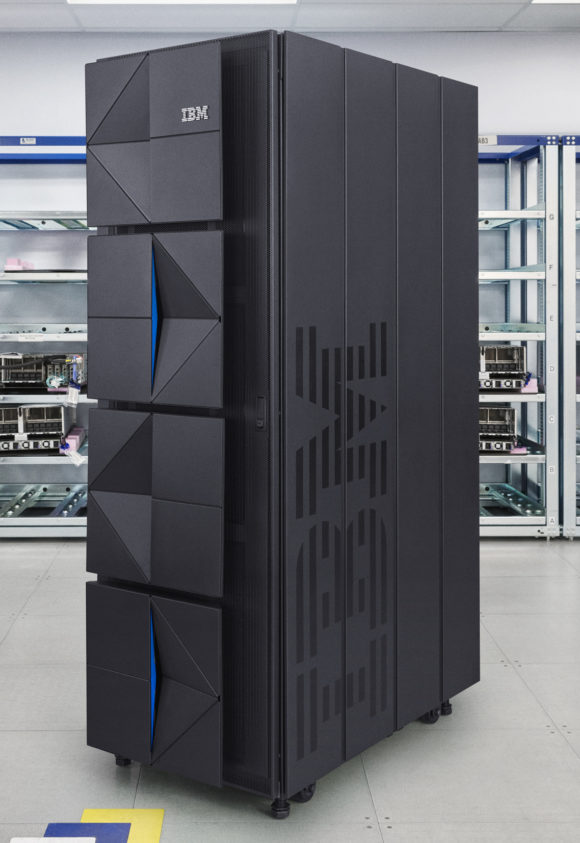
\includegraphics[width=0.40\linewidth]{bachproef//graphics/Singe_Frame_Mainframe_z16.jpg}
    \caption{Een single frame van een IBM z16 ~\autocite{Tech2023}}
    \label{fig:Een single frame van een IBM z16}
\end{figure}


Wanneer men tegenwoordig denkt aan mainframes denkt men vooral aan die van “the International Business Machines Corporation” beter bekend als IBM. IBM beheerst een gigantisch groot aandeel van de mainframe wereld wanneer het komt op beide hard- en software. In tegenstelling tot wat vaak wordt gedacht, heeft IBM de mainframe niet uitgevonden. Er waren alternatieven van andere fabrikanten, maar die zijn geleidelijk aan afgenomen, waarbij sommige bedrijven de productie zelfs volledig hebben stopgezet. Hoewel sommige bedrijven zoals Fujitsu, NEC, Unisys en Bull nog steeds eigen mainframes aanbieden, is het een afnemende markt volgens John Abbot~\autocite{DrewRobb}. Wanneer het aankomt op software heeft IBM wel meer competitie met software leveranciers zoals Broadcom en BMC al worden die producten grotendeels gebruikt op IBM’s eigen mainframes. Dit onderzoek wordt gedaan met een z16 IBM mainframe wat betekent dat vanaf dit punt verder het specifiek gaat over dat systeem tenzij anders vermeld.

\subsection{De eerste mainframes}
In dit deel van het onderzoek zal er besproken worden hoe we tot onze huidige situatie zijn geraakt wanneer het aankomt op mainframes. Want ze ondersteunen onze samenleving nu al decennia op een manier waarbij de bevolking weinig bewust contact men ze maakt. Om meer context te plaatsen op de huidige versies is het handig om eerst een blikje terug te nemen in het verleden. Het is hier niet de bedoeling dat men diepgaand een mainframe gaan onderzoeken. Een mainframe is zo breed dat dat buiten het scope van dit onderzoek valt. Er zullen dus hoogstwaarschijnlijk een aantal concepten of termen terugkomen dat iemand buiten de IT wereld niet meteen zou herkennen. Ze zijn niet belangrijk om dit onderzoek te begrijpen. Ze zou wel genoeg context moeten geven om te snappen dat een mainframe altijd blijft evolueren door nieuwe technologieen en/of concepten toe te passen. 

\subsection{z16}
De IBM z16 mainframe is in 2023 de meest recenste en geavanceerde systeem dat IBM heeft uitgebracht.Het is een aanzienlijke upgrade ten opzichte van de eerdere z15. De z16 maakt gebruik van de Telum-processor die draait op 5,2 GHz, dat is één van de snelste beschikbaar. Belangrijke verbeteringen zijn onder andere 17\% meer processor capaciteit per lade, een on-chip Accelerator for AI voor snelle AI-verwerking, en een herontworpen cache voor betere prestaties in transactionele scenario's. Het systeem behoudt een geheugencapaciteit van maximaal 40 TB met behulp van redundante array of independent memory (RAIM) technologie voor hoge beschikbaarheid. Connectiviteitsopties zijn uitgebreid en aanpasbaar aan verschillende behoeften. Door de verstaanbare behoeftes van zSystem klanten is veiligheid weer een topprioriteit, met quantum-safe mogelijkheden voor sleutelgeneratie en encryptie, evenals Pervasive Encryption voor het beveiligen van gegevens in rust en in transit. Het Security and Compliance Center is een nieuwe functie die compliance-taken vereenvoudigt. De z16 is een krachtige en veilige keuze voor bestaande IBM-mainframeklanten, met verbeteringen in prestaties, schaalbaarheid en beveiliging. Colruyt group gebruikt op dit moment deze versie van de IBM mainframes. Figuur 2.3 is een voorbeeld van een z16 mainframe met 4 frames.~\autocite{Laura2023,Steven2023}

\begin{figure}[h]
    \centering
    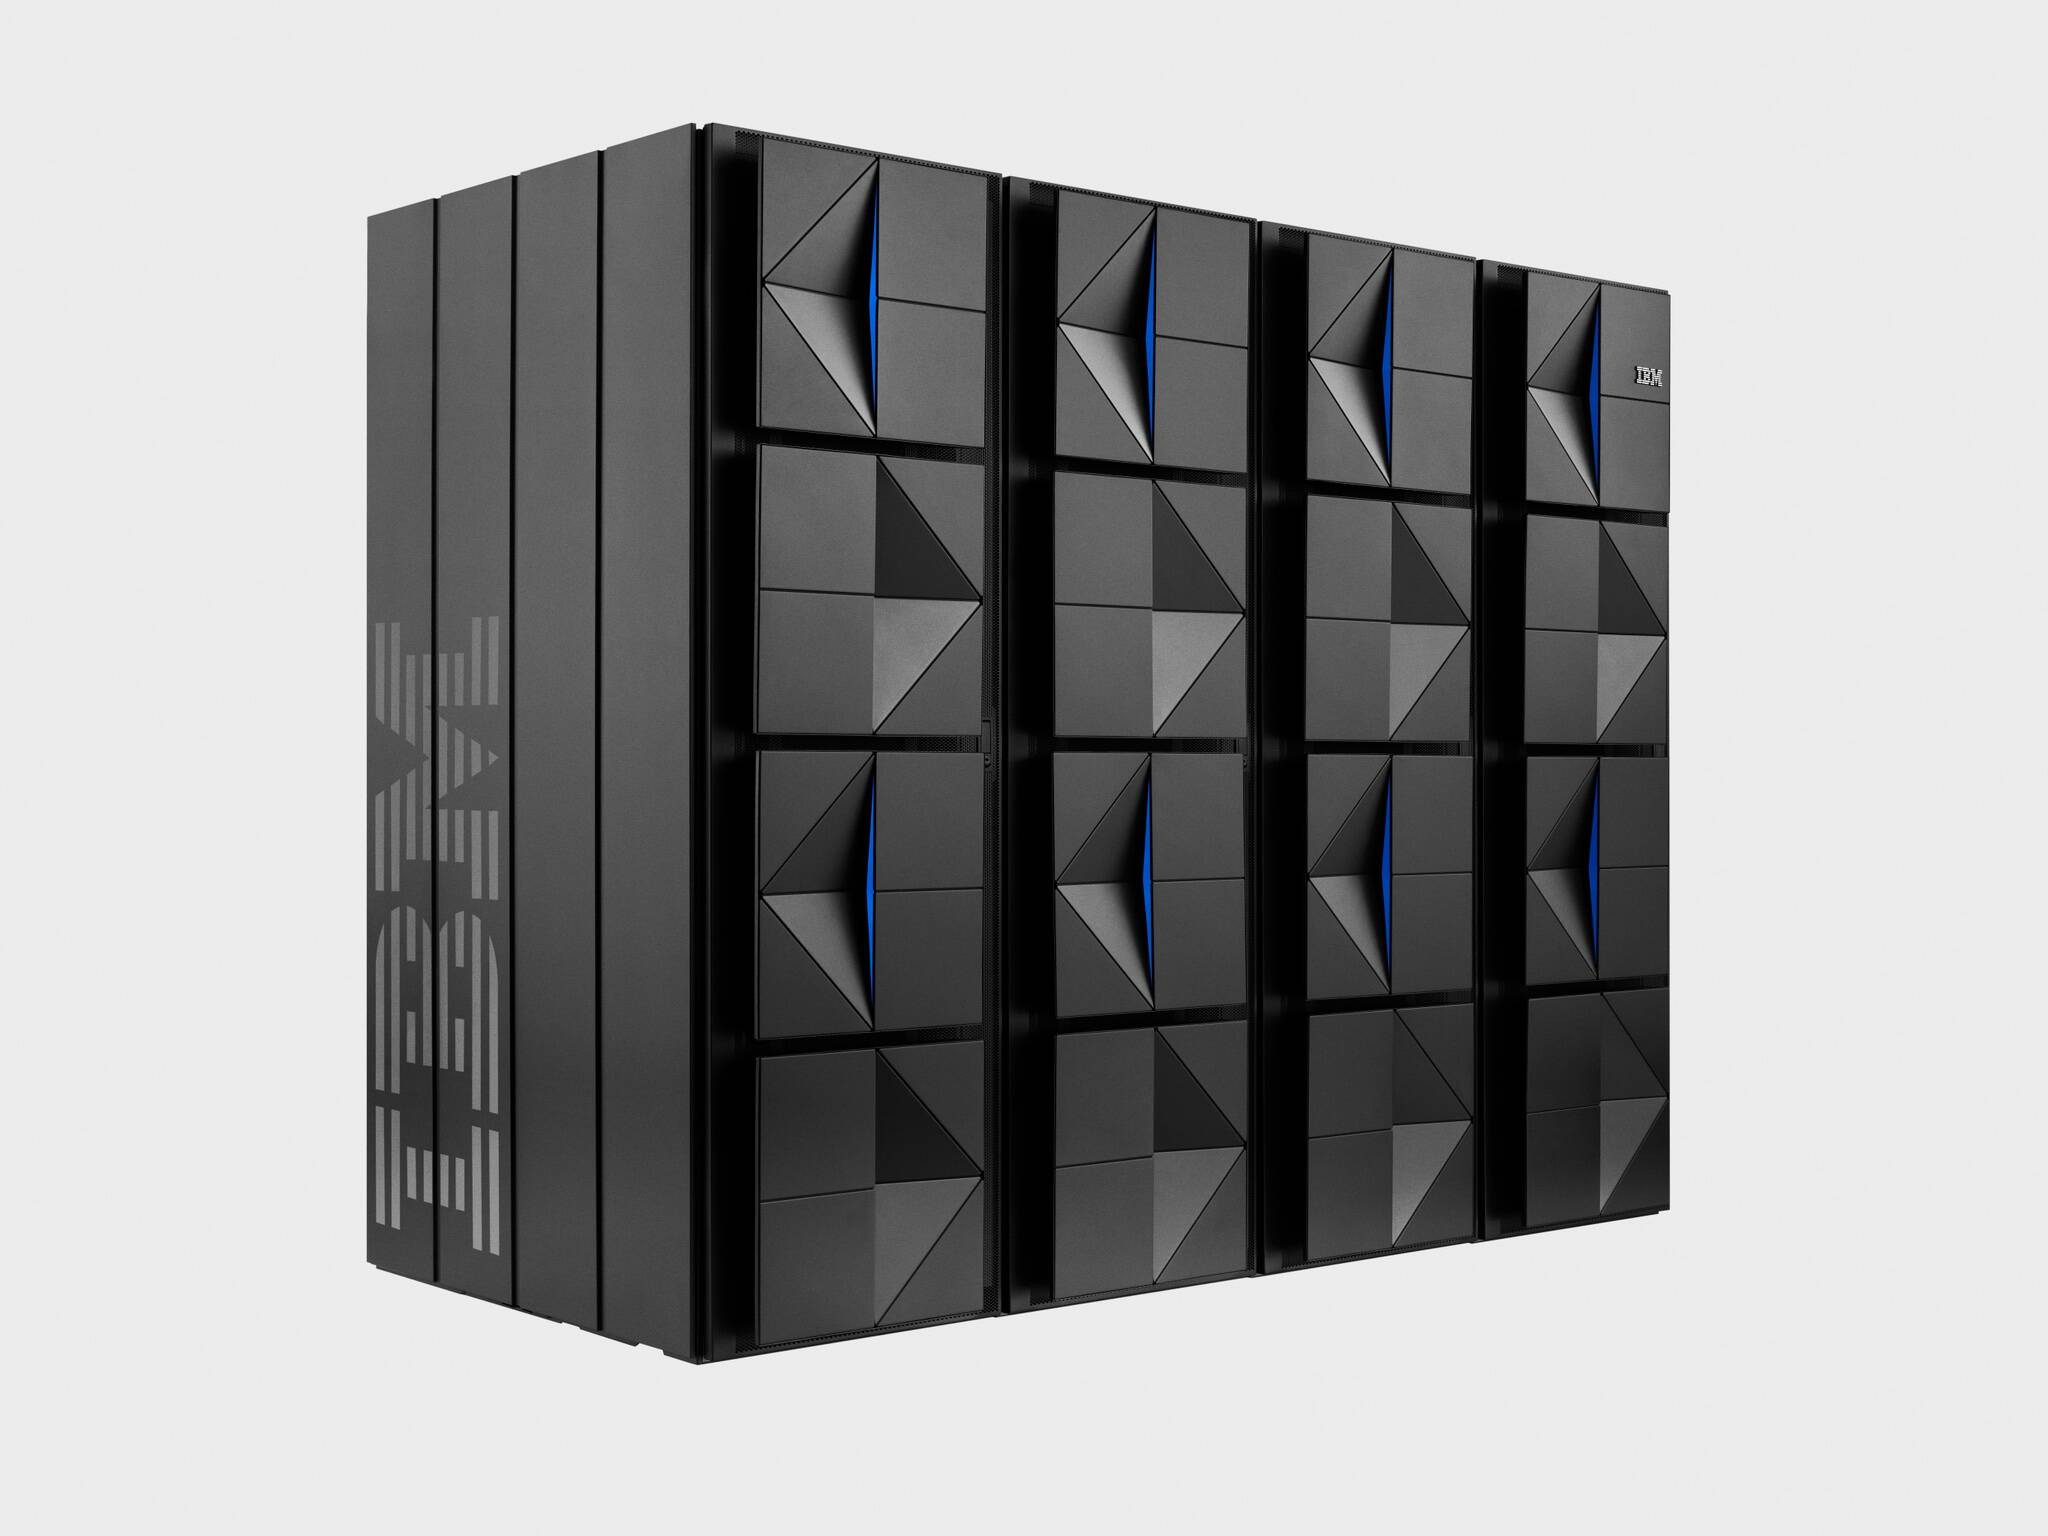
\includegraphics[width=0.5\linewidth]{bachproef//graphics/4-frame-z16.jpg}
    \caption{Een z16 met 4 frames ~\autocite{Elizabeth2022}}
    \label{fig:Een z16 met 4 frames}
\end{figure}

\subsection{Betrouwbaarheid}
Mainframes worden geprezen om hun ongeëvenaarde betrouwbaarheid. Deze betrouwbaarheid is gebaseerd op RAS-principes. RAS staat voor betrouwbaarheid (Reliability in het engels), beschikbaarheid (Availability in het engels) en Servicebaarheid. RAS zorgt voor zelfherstel van hardware en software, snelle foutcorrecties en minimale impact bij storingen. Hierdoor blijven mainframe consistent betrouwbaar en beschikbaar voor bedrijfstoepassingen. Dit doen ze op soft- en hardware niveau door zaken te voorzien zoals meerdere mogelijkheden om de mainframe van stroom te voorzien. Maar één van de belangrijkere concepten dat een mainframe toepast is het concept van een parrelel sysplex. Een parallel Sysplex is een technologie in de mainframe wereld die de betrouwbaarheid van systemen aanzienlijk verbetert. In tegenstelling tot gedistribueerde systemen, waar nodes onafhankelijk werken, stelt een parallel sysplex meerdere mainframesystemen in staat om samen te werken als een geheel. Deze samenwerkingsaanpak biedt verschillende voordelen op het gebied van betrouwbaarheid. Aangezien dat meerder mainframestystemen aanzienlijk ver van elkaar kunnen staan en toch perfect nog kunnen samenwerken. Ook worden gegevens meestal gelijk gehouden tussen machines. Dit zorgt ervoor dat als er een machine toch zou uitvallen dat een bedrijf of organisatie toch kan blijven draaien.~\autocite{FrankJDGilio,maincom,Subhasish2020}
De IBM z16 is een recente toevoeging aan deze traditie van betrouwbaarheid, met een uptime van 99.9999999\%. Dit komt neer op slechts iets meer dan 30 milliseconden downtime per server per jaar. Uit ervaring weet men dat er mainframes draaien die al jaren geen downtime hebben gehad. Deze ongeëvenaarde betrouwbaarheid maakt mainframes ideaal voor kritische toepassingen in de moderne zakelijke omgeving. Dit maakt mainframes tot een dominante keuze voor bedrijven die uptime en betrouwbaarheid in hoge belangstellen. Dus in conclusie is betrouwbaarheid één van de kernconcepten van mainframes. Zo'n kernconcept dat de "z" in z16 staat voor zero downtime. ~\autocite{IBM2023(3),JasonBloomberg,RobEnderle}

\subsection{Systeem logs}
 Wat hier nog niet besproken is geweest zijn de mainframe werknemers die er voor zorgen dat problemen opgelost of voorkomen worden. Dat is uiteraard ook een essentieël onderdeel om de mainframe standarden in betrouwbaarheid hoog te houden. Een dat de mainframe ervoor zorgt dat die werknemers hun job kunnen doen is door extensieve logs mee te geven. De log waar in dit onderzoek jet over gaat is de "SYSLOG". Systeemlogs op een mainframe zijn gegevens die worden gemaakt door het besturingsysteem en een sommige softwarecomponenten om informatie meetegeven over hun werking en enige problemen dat ze ondervinden. Ze zijn essentieel voor oplossen van problemen, onderhouden en monitoren van het systeem. Bij Colruyt Group lopen deze logs starten om zes uur 's ochtends en lopen 24 uur. Tijdens deze periode worden de logs geschreven naar een active logs om dan na 24u te worden opgeslaan en geachriveerd.
 
\subsection{JCL}
JCL,Job Control Language voluit, is een essentieel onderdeel van de mainframe en dient als communicatiemiddel tussen programma's zoals COBOL en PL/I en het besturingssysteem. Het speelt een belangrijke rol bij het uitvoeren van batch- of online verwerking. Bij batchverwerking kunnen taken bijvoorbeeld bestaan uit het verwerken van grote hoeveelheden banktransacties. Bij online verwerking daarentegen vinden real-time interacties plaats, zoals bankmedewerkers die een back-officescherm gebruiken om rekeningen te openen.Het is een soort programeertaal dat de mainframe zegt welke stappen die moet zetten om de job succesvol ui te voeren.~\autocite{tutpoint} Hier zijn stappen voor verwerken van taken met behulp van JCL:

\subsubsection{Taakinvoer}
Gebruikers dienen JCL in bij het Job Entry System (JES) van het besturingssysteem. Dit is waar alle jobs binnenkomen en voorbereid worden om uit te voeren.

\subsubsection{Taakconversie}
JCL, samen met eventuele bijbehorende procedures , worden omgezet in een interpreteerbaar formaat voor JES en wordt opgeslagen in een dataset genaamd SPOOL.

\subsubsection{Taakwachtrij}
JES bepaalt de prioriteit van taken op basis van parameters zoals CLASS en PRTY die zijn gedefinieerd in de job. Het controleert ook op fouten en steekt de job in de wachtrij als er geen fouten zijn.

\subsubsection{Taakuitvoering}
Wanneer een taak de hoogste prioriteit bereikt, wordt deze uit de wachtrij gehaald voor uitvoering. Het programma wordt uitgevoerd vanuit de SPOOL en de uitvoer wordt doorgestuurd naar de bestemming dat gespecifieerd werd in de job.

\subsubsection{opkuisen}
Na dat alles klaar is worden de toegewezen middelen vrijgegeven. De joblog wordt uit de SPOOL verwijderd dus als men die wilt oplsaan moet die naar een dataset weggeschreven worden.

\subsection{Service now}
ServiceNow is een cloudgebaseerd IT Service Management platform dat processen automatiseert. Service Now voldoet aan ITIL-richtlijnen voor servicegerichte operaties. Het maakt gebruik van machine learning voor efficiëntie en schaalbaarheid. Belangrijke functies omvatten onder andere  kosteneffectieve ondersteuning, aanpasbaarheid en gegevensbeveiliging. Binnen Colruyt Group en voor dit onderzoek wordt Service now voornamlijk gebruikt om ticketten aan te make om problemen op te lossen of producten te leveren. ~\autocite{DavidTaylor}

\section{ELK}
ELK is een groep van voormalige open-source software applicaties dat samenwerken om de ELK-stack te vormen. Er zijn drie hoofdapplicaties dat een ELK-stack maken en die zijn Elasticsearch, Logstash en Kibana. Daarbij komen soms andere applicaties zoals Beats ook bij kijken. Gemaakt en beheerd door Elastic, ELK dient om logs te analyseren en te visualiseren. Zo kunnen teams niet alleen hun logs overzichtelijk bekijken maar ook grafieken maken en vergelijken met vorige logs ofdat er iets verschilt. In dit hoofdstuk gaat er gekeken worden naar alle ELK componenten die van toepassing gaan komen tijdens dit onderzoek. Figuur 2.5 ~\autocite{DavidTaylor} geeft al een klein overzicht van hoe ELK werkt.~\autocite{DavidTaylor,DotanHorovits}


\begin{figure}[h]
    \centering
    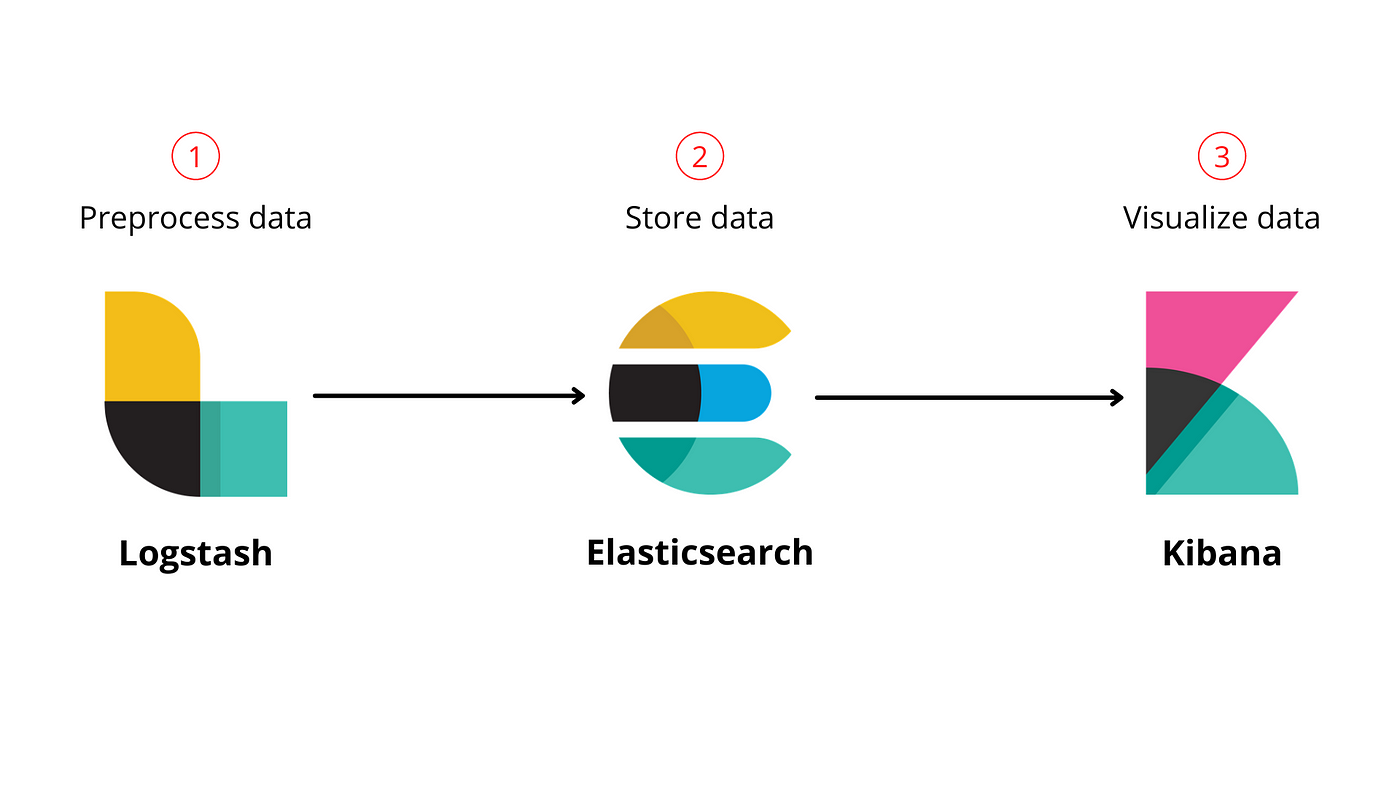
\includegraphics[width=0.5\linewidth]{bachproef//graphics/ELK_stack_essentials.png}
    \caption{Een ELK-stack met alleen de essentials ~\autocite{DavidTaylor}}
    \label{fig:Een ELK-stack met alleen de essentials}
\end{figure}

\subsection{Elastisearch}
Elasticsearch is een prominente NoSQL-database gebouwd op de krachtige Lucene-zoekmachine, bekend om zijn robuuste mogelijkheden op het gebied van gegevensopslag en -opvraging. ELk is een zoekserver is geschreven in Java en het blinkt uit in het indexeren van heterogene gegevenstypen. Elasticsearch werkt binnen een cluster, dat een verzameling nodes vertegenwoordigt die gegevens vasthouden en indexerings- en zoekmogelijkheden bieden. Nodes vertegenwoordigen individuele Elasticsearch-instanties. Gegevens zijn georganiseerd in indexen, die elk vergelijkbare documenten bevatten. Documenten worden geïndexeerd en geassocieerd met een unieke ID. Indexen kunnen worden verdeeld in shards voor distributie, en de schaalbaarheid van Elasticsearch kan worden bereikt door meer nodes aan het cluster toe te voegen. Het biedt een REST API-webinterface met JSON-uitvoer, wat integratie in verschillende toepassingen vergemakkelijkt. Elasticsearch biedt ondersteuning voor meerdere talen aan naast functies zoals volledige tekstzoekopdracht, bijna-realtime (NRT) zoekopdracht, sharding, replicatie.Een van de belangrijke voordelen is het vermogen om gegevens zonder een schema te verwerken, waardoor gebruikers gegevens record voor record kunnen manipuleren met multi-document API's. Daarnaast staat Elasticsearch bekend om zijn schaalbaarheid, zowel verticaal als horizontaal. Het ondersteunt verschillende programmeertalen dankzij de beschikbaarheid van pogammeertalen. ~\autocite{GedalBer}  

\subsection{Logstash}
Logstash is een gegevensverwerkingstool die oorspronkelijk is ontworpen voor log-analyse, maar zich heeft ontwikkeld tot een veelzijdige gegevensverwerkingstool. Het werkt als een pijplijn in 3 fases: invoer, filter en uitvoer.~\autocite{Jamie2017,JugensToit}  

\subsubsection{invoerstadium}
In het invoerstadium verzamelt Logstash gegevens uit verschillende bronnen, waaronder logbestanden, netwerkprotocollen en wachtrijen. Het kan inkomende gebeurtenissen taggen met metagegevens die verband houden met hun bron.

\subsubsection{filterstadium}
Het filterstadium in Logstash voegt aanzienlijke waarde toe door middel van filter-plugins. Deze plugins zijn verantwoordelijk voor het transformeren en verrijken van gegevens. Ze kunnen voorwaardelijke logica toepassen op basis van eigenschappen van gebeurtenissen, velden extracten en bewerkingen uitvoeren zoals het parseren van tijdstempels en het omzetten van gegevenstypen. Het correct rangschikken van deze filter-plugins is van cruciaal belang om een efficiënte gegevensverwerking te verzekeren.

\subsubsection{uitvoerstadium}
Het uitvoerstadium handelt de levering van verwerkte gebeurtenissen naar verschillende bestemmingen af, zoals databases, wachtrijen, API's en meer. Logstash ondersteunt meerdere uitvoerkanalen voor een enkele gebeurtenis, waardoor het zeer aanpasbaar is voor verschillende use-cases. Logstash biedt ook codecs, die bepalen hoe gegevens worden geserializeerd of gedeserialiseerd. Codecs zijn bijzonder nuttig voor het verwerken van gestructureerde gegevensformaten zoals JSON of meerregelige logvermeldingen.Wat betreft architectuur kan Logstash worden ingezet in verschillende configuraties, van single-server configuraties tot complexe gedistribueerde infrastructuren. De keuze voor de architectuur hangt af van de schaal en de vereisten voor log-verwerking.Logstash is een fundamenteel onderdeel in Extract-Transform-Load (ETL) pijplijnen gewirden, waarbij gegevens effectief worden verwerkt uit diverse bronnen en formaten.

\subsection{Kibana}
De K van ELK staat voor Kibana het programma dat verantwoordelijk is voor visualisatie en analysatie. Het interface dat toegang geeft aan de visualisatie mogelijkheden van Kibana is in dashboard formaat. Een ELK-dashboard bestaat uit verschillende panelen dat de gebruiker zelf kan instellen.~\autocite{Elatic(1)} Figuur 2.5 is een voorbeeld van een dashboard. Een paneel kan uitvolgende soorten bestaan:

\begin{itemize}
    \item Editors
        Editors is een collectie van panelen die onderandere dienen om grafieken weer te geven. Voorbeelden zijn tabbellen, heatmap en treemaps. 
    \item Maps
        Het doel van deze panelen is om geografische kaarten te maken van de beschikbare gegevens.

    \item Anomaly swim lane
        Met deze paneel kan een gebruiker naar de resulaten van de anomaly detection kijken. Meer over Anomaly detection later.
        
    \item Anomaly chart
       Deze paneel geeft de gebruiker de mogelijkheid om een grafiek van anomalies te zien.
        
    \item Log stream
        Deze paneel dient om de huidige logs te zien dat ELK binnenkrijgt.

    \item Tools
        Deze paneel geeft de mogelijk om interactieve filter mogelijkheden te maken. Een voorbeeld hiervan is time slider dat u de optie geeft om te filteren op een start en eind tijd.

    \item Text
        Met deze paneel kan u makkelijk tekst toevoegen aan uw dashboard. Dit kan handig zijn om documentatie of instructies te schrijven.

    \item Image
        Om uw dashboard te kunnen personaliseren is er ook een mogelijkheid om foto's of logo's op uw dashboard te zetten. Dit kan met foto's van op uw computer of externe links.
\end{itemize}


\begin{figure}[h]
    \centering
    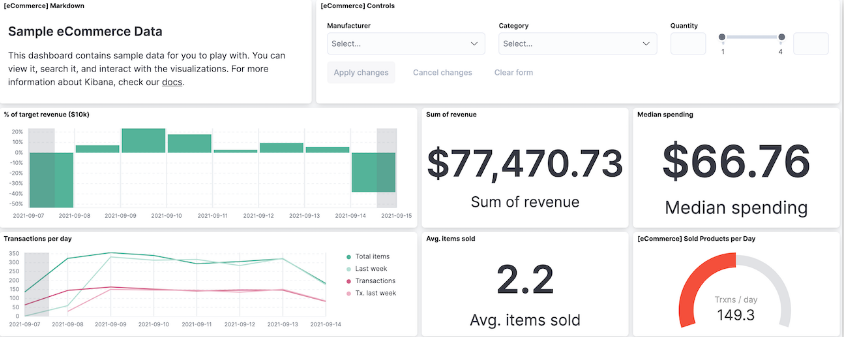
\includegraphics[width=0.75\linewidth]{bachproef//graphics/Voorbeeld_Dashboard.png}
    \caption{Een voorbeeld van een ELK dashboard ~\autocite{Eleanor2023}}
    \label{fig:een voorbeeld van een ELK dashboard}
\end{figure}

\subsection{Beats}
Zoals eerder vemeldt is geweest kunnen er naast de drie ELK-programma's andere programma's ELK ondersteunen. Onder deze programma's is het Beats-ecosysteem bijzonder opmerkelijk en de meest voorkomende. Beats zijn in wezen lichtgewicht agenten die zijn ontworpen voor specifieke taken voor gegevensverzameling en die verzamelde gegevens overdragen naar Elasticsearch. Zulke applicaties worden wel 'data-shippers' genoemd. Wanneer men Beats toevoegt aan ELK spreekt men dan meestal van een Elastic-stack. De sleutel tot de veelzijdigheid van Beats ligt in het libbeat-framework. Dit framework vereenvoudigt het maken van aangepaste gegevens verzamelingsagents, waardoor het haalbaar is om Beats aan te passen aan verschillende soorten gegevens. Als gevolg daaraan blijft het Beats-ecosysteem snel groeien. Op dit moment zijn er zes officiële Beats ontwikkeld door Elastic. Deze Beats zijn open source en vallen onder de Apache-licentie. Samen pakken ze het veelvoorkomende probleem aan van het efficiënt verzamelen van gegevens en het doorsturen ervan naar Elasticsearch.~\autocite{objectrocket}  

\subsubsection{Filebeat}
eerst ontworpen voor het lezen van bestanden vanuit het systeem, is Filebeat met name handig voor het verwerken van systeem- en toepassingslogbestanden. Het stroomlijnt de centralisatie van logs door logs van verschillende servers en Virtuele machines te lezen en door te sturen naar een centrale Logstash- of Elasticsearch-instantie. Daarnaast vereenvoudigt Filebeat de configuratie met vooraf gebouwde modules voor veelvoorkomende logbestandsindelingen.

\subsubsection{Metricbeat}
Metricbeat specialiseert zich in het verzamelen van metingen van servers en systemen, wat ideaal is voor het monitoren van systeem- en service-statistieken. Net als Filebeat bevat Metricbeat modules voor verschillende besturingssystemen en toepassingen, wat zorgt voor minimale impact op systeemprestaties.

\subsubsection{Packetbeat}
Packetbeat fungeert als een lichtgewicht netwerkpacketanalyzer en bewaakt continu netwerkprotocollen om inzicht te bieden in netwerklatentie, fouten, responstijden en meer. Het ondersteunt meerdere toepassingslaagprotocollen.

\subsubsection{Winlogbeat}
Speciaal ontworpen voor Windows-omgevingen, levert Winlogbeat live streams van Windows-logboek gebeurtenissen. Het bewaakt verschillende gebeurtenissen, zoals aanmeldingen, USB-apparaatgebruik en software-installaties, en stuurt deze gegevens door naar Elasticsearch voor beveiligingsmonitoring.

\subsubsection{Auditbeat}
Voor Linux-platforms voert Auditbeat een gelijkiaardige functie uit door gebruikers- en procesactiviteit over het systeem te bewaken. Audit-gegevens worden in realtime naar Elasticsearch verzonden voor beveiligingsmonitoring.

\subsubsection{Heartbeat}
Heartbeat kan systemen pingen om te zien of ze nog operationeel zijn. Deze info wordt dan naar ELK gestuurd. Het ondersteunt meerdere protocollen en functies, waaronder TLS, verificatie en proxies, en lost efficiënt DNS op om hosts achter load-balanced servers te monitoren.


\begin{figure}[h]
    \centering
    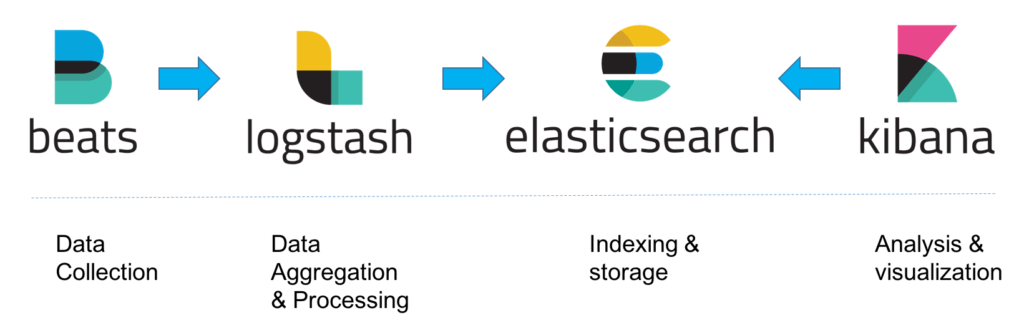
\includegraphics[width=0.5\linewidth]{elk_stack_beats.png}
    \caption{Een ELK-stack met beats ~\autocite{DavidTaylor}}
    \label{fig:Een ELK-stack met beats}
\end{figure}

\subsection{Anomaly detection}
Ook staan we even stil bij deviatie detectie functies dat Elastic aanbiedt. Dat is een live hulpmiddel binnen de Elastic Stack dat bedoeld is om afwijkingen in tijdreeksgegevens te identificeren. Het leert autonoom de normale patronen en trends in de gegevens, vermindert valse alarmen en vereenvoudigt de analyse van de onderliggende oorzaken. Deze functie zou erg van pas komen voor MFPOSS. Belangrijke onderdelen zijn:
\begin{itemize}
    \item Jobbeheer voor het maken en beheren van taken voor deviatie detectie.
    \item Kalenderbeheer voor aangepaste regels.
    \item Visualisatietools zoals de deviatie-verkenner en de Weergave van enkele metrieken.
    \item Handmatige of automatische annotaties toevoegen aan afwijkingen voor context.*
    \item Het Jobbeheerpaneel houdt een uitgebreide lijst van annotaties bij voor elke taak.
\end{itemize}


Al deze onderdelen helpen bij het volgen van afwijkingen en het verbeteren van de operationele werkingen.
*Automatische annotaties worden toegevoegd voor situaties zoals ontbrekende gegevens. ~\autocite{Elatic(2)} 

\section{DataDog}

\section{Grafana}

\section{Linux}

\subsection{Linux Server}

\subsection{RedHat}

\subsection{FTP}